%%%%%%%%%%%%%%%%%%%%%%%%%%%%%%%%%%%%%%%%%%%%%%%%%%%%%%%%%%%%%%%%%%%%%%%%%%%%%%%%%%%%%%%%%%%
\section{Simulation study}\label{sec:sim}
%%%%%%%%%%%%%%%%%%%%%%%%%%%%%%%%%%%%%%%%%%%%%%%%%%%%%%%%%%%%%%%%%%%%%%%%%%%%%%%%%%%%%%%%%%%

In this section we test procedure in Algorithm~\ref{alg:hotcold}, identify its characteristics, properties, and also compare it  with standard hot-spot methods on data where the true hot and cold areas are known. All code is available in the repository of the \texttt{hotcoldESF} package, \url{https://github.com/yandiracuvero/hotcoldESF}, archived on Zenodo \citep{hotcoldesf2026}. 
%, and to check the choices of Section~\ref{sec:rationale}. 

\subsection{Design}\label{sec:sim-design}

%\paragraph{Point patterns.}
 Points are generated in the square window $[0,1000]^2$. Every pattern contains three components:
\begin{itemize}
  \item 2000 points distributed uniformly (background);
  \item 3000 points whose intensity follows an environmental covariate: a Gaussian bump $b(u)=\exp\{-\lVert u-u_0\rVert^2/(2\cdot150^2)\}$ centred at a random location $u_0$ away from the clusters, with points accepted with probability $\exp\{3(b(u)-1)\}$;
  \item clusters, generated as a modified Thomas process: each cluster has a centre and a fixed number of points distributed uniformly within a disc (or an ellipse) around it.
\end{itemize}
The covariate area is part of the explained variation: the model receives the covariate $b$ evaluated at the centre of each cell, together with an irrelevant covariate drawn from a standard normal distribution. A method that adjusts for covariates should not label the covariate area as hot.

%\paragraph{Scenarios.} 
Table~\ref{tab:scenarios} lists the scenarios concidered. Scenarios B, L, E, M and S vary the size, shape and number of the clusters; K adds a true cold area, where only a fraction of the points is kept; U has the same data as B but the model does not receive the covariate, to show the effect of a missing covariate; C and N contain no clusters. Every scenario except C and N has a weak and a strong clustering version.

\begin{table}[ht]
\centering
\caption{Simulation scenarios. All patterns also contain 2000 uniform points and 3000 points that follow the covariate; the window is $1000\times1000$.}\label{tab:scenarios}
\small
\begin{tabularx}{\textwidth}{l>{\raggedright\arraybackslash}X>{\raggedright\arraybackslash}X>{\raggedright\arraybackslash}p{3.2cm}}
\toprule
Scenario & Clusters & Points per cluster (weak / strong) & Purpose \\
\midrule
B & 3 discs, radius 100 & 50 / 200 & compact clusters \\
L & 2 discs, radius 200 & 200 / 600 & large, diffuse clusters \\
E & 3 ellipses, semi-axes $300\times33$ & 100 / 300 & elongated clusters \\
M & 3 discs, radii 50, 100, 200 & same intensity: 24, 94, 377 / 50, 200, 800 & clusters of different sizes \\
S & 8 discs, radius 40 & 15 / 40 & many small clusters \\
K & as B (200 points) & cold disc of radius 150 keeps 50\% / 20\% & a true cold area \\
U & as B & 50 / 200; covariate not given to the model & missing covariate \\
C & none & -- & covariate area only \\
N & none & 3000 uniform points, no covariate area & complete spatial randomness \\
\bottomrule
\end{tabularx}
\end{table}

%\paragraph{Grids.} 
Points are counted on a $20\times20$ grid (cell side 50) and on a $40\times40$ grid (cell side 25), with queen contiguity. We generate 100 datasets per setting on the $20\times20$ grid and 50 on the $40\times40$ grid, 2400 datasets in total. The permutation band uses $B=999$ permutations on both grids, as in the application.

%\paragraph{Methods.} 
The proposed procedure (Algorithm~\ref{alg:hotcold}, denoted ESF) is compared with:
\begin{itemize}
  \item Getis-Ord $G_i^*$ \citep{getis1992analysis,ord1995local} on the residuals $u$ of $\log(1+w)$ on the covariates, with binary weights including the cell itself; a cell is hot if $G_i^*>1.645$ and cold if $G_i^*<-1.645$. We consider three versions: alone, preceded by the test of Step~1, and preceded by the test with a false discovery rate correction \citep{benjamini1995controlling};
  \item local Moran's $I$ (LISA) \citep{anselin1995local} on the same residuals, with conditional permutation $p$-values (999 permutations) and preceded by the test; a cell is hot if it is high--high with $p<0.05$, cold if low--low with $p<0.05$;
  \item two rankings without spatial smoothing: the cells with the largest residuals $u$ (top residuals) and the cells with the largest counts (top counts).
\end{itemize}
The $G_i^*$ ranking orders cells by $G_i^*$, and the LISA ranking orders high--high cells by their local $I$.





\subsection{Choices within the procedure}\label{sec:sim-choices}

The choices listed below rest on three sources of evidence. Choices~\ref{ch:log}, \ref{ch:cand}, \ref{ch:ridge} and~\ref{ch:band} were made with preliminary experiments, run before the main study on scenarios A (three clusters of 500 points and 2000 uniform points, no covariate area), B, C and N and on the same two grids (and a $10\times10$ grid for choice~\ref{ch:log}). Choices~\ref{ch:cov}, \ref{ch:test} and~\ref{ch:esf} are supported by the main study, whose results are reported in Section~\ref{sec:sim-results}; for choice~\ref{ch:cov}, the preliminary experiments also applied $G_i^*$ and local Moran's $I$ to the counts. Choice~\ref{ch:lin} comes from a further analysis of 900 datasets of the main study (scenarios B, S and C), refitted with a natural spline for each covariate. The scripts and full results are in the repository.

%\subsection{Rationale for each step}\label{sec:rationale}
%Each choice above was compared with alternatives in the simulation study of Section~\ref{sec:sim}. We summarise the reasons here.

Each item below refers to the line of Algorithm~\ref{alg:hotcold} and the step of Section~\ref{sec:met} that it justifies.

\begin{enumerate}

\item\label{ch:log} \textbf{Logarithm of the counts} (Algorithm~\ref{alg:hotcold}, line~\ref{alg:l-data}: $y\gets$ standardised $\log(1+w)$; Step~1).
Counts of sightings are skewed and their variance grows with the mean, so a few cells with many reports dominate a model for the raw counts. On the log scale, the test of Step~1 correctly finds no spatial structure when the pattern is fully explained by a covariate; on the raw scale it does not.

\item\label{ch:cov} \textbf{Covariate adjustment} (line~\ref{alg:l-data}: $X\gets(\mathbf{1},Z)$ and $u\gets M_Xy$; Step~1).
Without covariates, a hot spot is simply an area with many sightings, and areas where the environment favours the pest are flagged even when nothing else is going on. In the simulation study, ranking cells by their counts (or applying Getis-Ord $G_i^*$ and local Moran's $I$ to the counts) placed most of the selected cells in an area driven by a covariate: the share of the top 5\% of cells inside a true cluster was at most 0.32, and close to zero with weak clusters.

\item\label{ch:lin} \textbf{Linear covariate terms} (line~\ref{alg:l-data}: the columns of $X$; Step~1).
A natural spline with 2 to 4 degrees of freedom for each covariate reduced the false rejections of the test in scenario C from 19--32\% to 4--6\%, but also reduced the rejections with weak small clusters (S) from 64--76\% to 28--44\%: a flexible function of a smooth covariate absorbs part of the cluster signal \citep{hodges2010adding}. We keep linear covariate terms and report the spline version as a sensitivity analysis.

\item\label{ch:test} \textbf{Test before mapping} (line~\ref{alg:l-test}; Step~1).
Local statistics label some cells as hot even when there is no clustering at all: at the 5\% level, about one cell in twenty. Testing the residuals first removes most of these false hot cells: in the simulation study, $G_i^*$ labelled 4.0--5.6\% of the map hot when there were no clusters, and 0.2--1.9\% when it was preceded by the test (Table~\ref{tab:sim-labels}), without any change in its ranking. %The same test can be placed in front of any local statistic, and we do so for the benchmarks.

The test does not depend on how the cells are labelled afterwards, so it can be used as a
first step for any local statistic. In the simulation study we also apply it to the
benchmarks ($G_i^*$ and local Moran's $I$), so that differences between methods in the
number of false hot cells come from the local statistic and not from the test.

\item\label{ch:esf} \textbf{Eigenvector spatial filtering} (lines~\ref{alg:l-cand}--\ref{alg:l-fit}; Step~2).
ESF estimates the spatial component inside a regression, so the covariates are adjusted for in the same model, and it represents patterns at several scales at once. Local statistics such as $G_i^*$ average each cell with a fixed neighbourhood. In the simulation study this difference matters when clusters of different sizes coexist: ESF finds the smaller clusters more often.

\item\label{ch:cand} \textbf{Smooth candidates} (line~\ref{alg:l-cand}: $\mathcal{C}\gets\{j:\delta_j\ge c\,\delta_1\}$; Step~2, equation~\eqref{eq:candidates}).
Eigenvectors with small or negative eigenvalues describe patterns that alternate between neighbours and fit cell-level noise. Restricting the candidates to~\eqref{eq:candidates} improved the precision of the top-ranked cells mainly where it was low: with weak clusters and on the finer grid it roughly doubled (for example from 0.17 to 0.36 with cross-validated penalties), with little change elsewhere.

\item\label{ch:ridge} \textbf{Ridge with a cross-validated penalty} (line~\ref{alg:l-fit}: choice of $\lambda$ and of the estimator; Step~2, equation~\eqref{eq:ridge}).
We compared eight ways to choose the penalty (the Moran's $I$ Lasso rule $|z_0|^{-a}$ with $a=1,2,3,4$; cross-validation with the smallest error and with the one-standard-error rule; BIC; and the largest penalty whose residuals pass the Moran test), each with all eigenvectors or with the smooth candidates~\eqref{eq:candidates}. The rule $|z_0|^{-2}$ of the Moran's $I$ Lasso \citep{barde2023moran} has good properties for estimating $\beta$ \citep{barde2024moran}, but for mapping $f$ it ties the amount of smoothing to the strength of the Moran signal: with weak clusters ($|z_0|\approx3$) the penalty is large and often no eigenvector is selected, so $\hat f=0$; with strong clusters ($|z_0|>10$) it is so small that almost all eigenvectors enter and $\hat f$ follows the noise. With this rule and all eigenvectors, the precision of the top 5\% with weak clusters was 0.19 ($20\times20$) and 0.11 ($40\times40$): the Lasso selected no eigenvector in 6 of 17 datasets with residual structure. Cross-validation with smooth candidates raised these values to 0.52 and 0.36 while keeping 0.98--1.00 with strong clusters, and replacing the Lasso by ridge, which keeps all smooth candidates instead of selecting a few, raised them further to 0.67 and 0.47. Our aim is to map $f$, not to select eigenvectors consistently, so the theoretical reservations about cross-validation for variable selection \citep{clc21} do not apply here. Spatial (block) folds for the cross-validation did not change the results, which is consistent with the near-uniform shrinkage described after~\eqref{eq:fhat}. Figure~\ref{fig:penalty} summarises the comparison: rules that penalise little ($|z_0|^{-3}$, $|z_0|^{-4}$) do well with weak clusters but lose precision with strong ones, rules that penalise more ($|z_0|^{-1}$, the one-standard-error rule, BIC) fail with weak clusters, and cross-validation with smooth candidates is the only Lasso rule that does well in both; ridge improves on it with weak clusters.

\begin{figure}[ht]
\centering
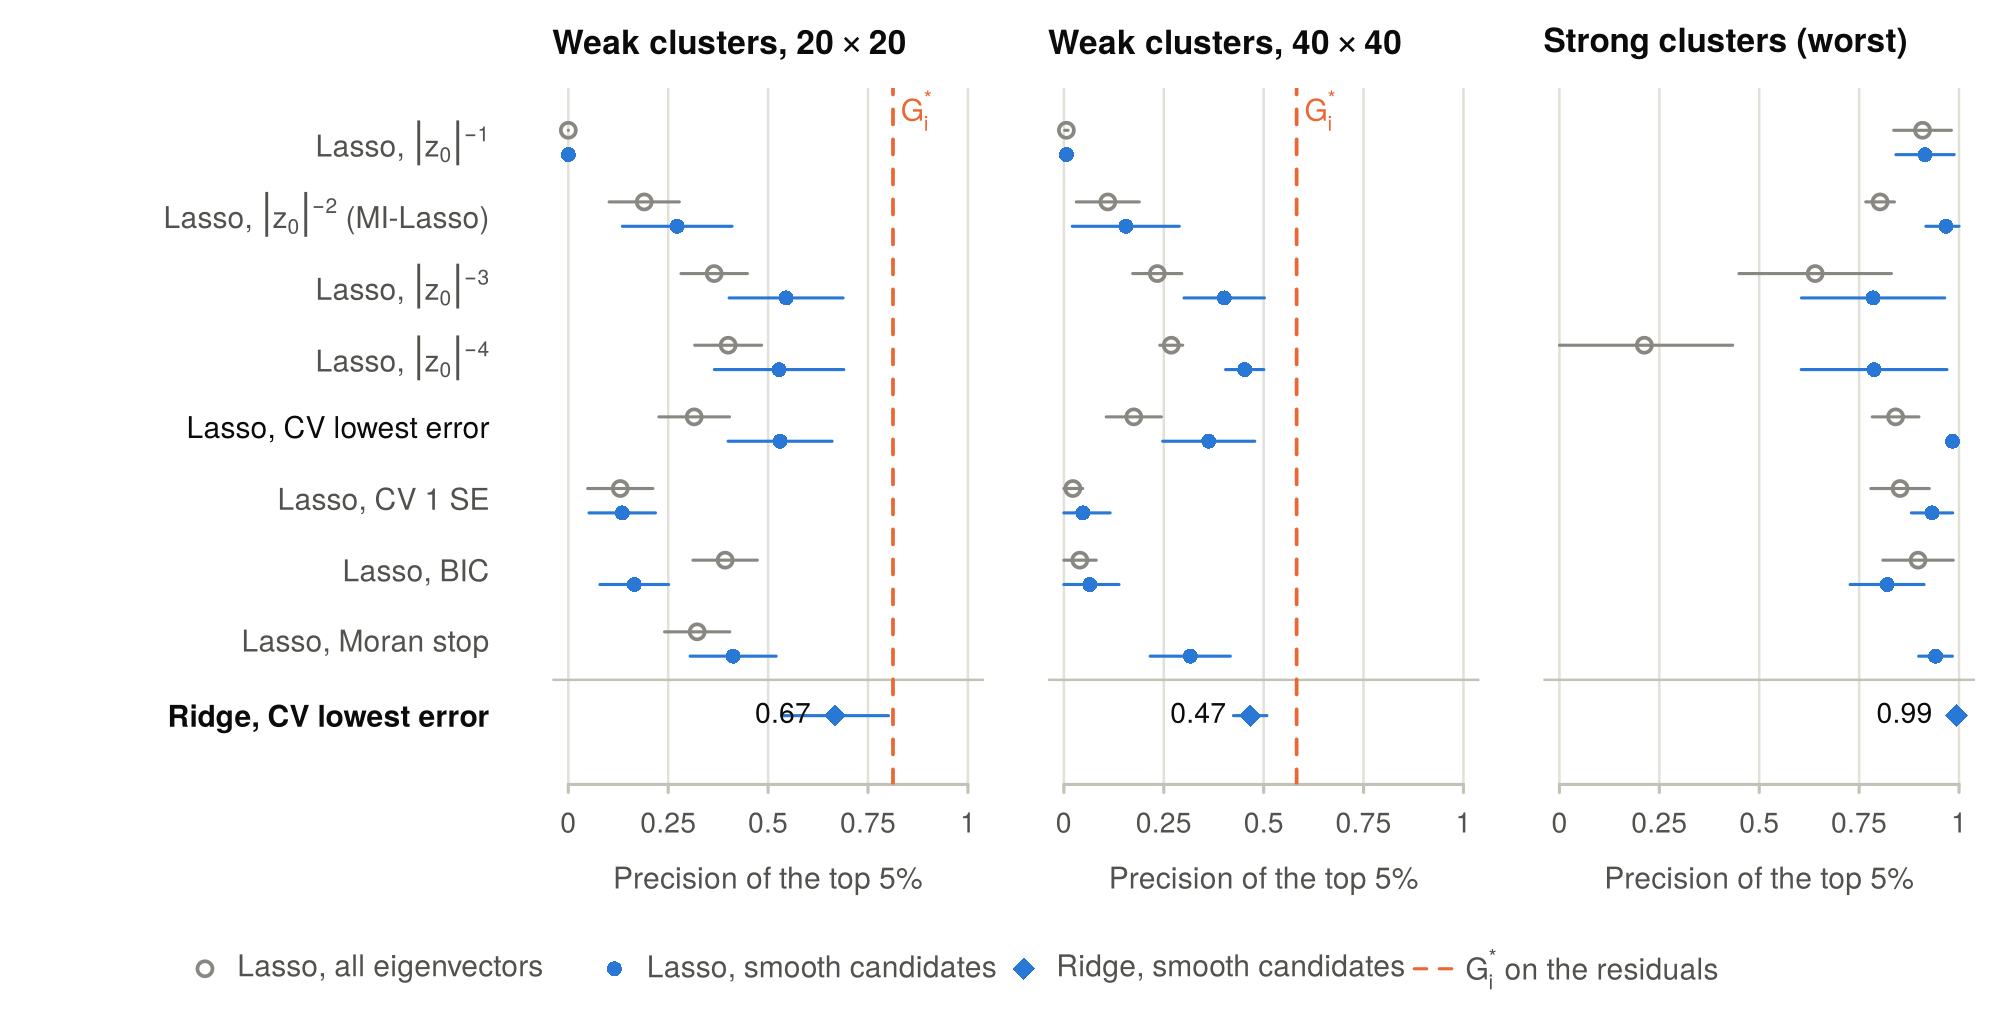
\includegraphics[width=\textwidth]{fig17_penalty_choice.png}
\caption{Choice of the estimator and of the penalty in Step~2 (choice~\ref{ch:ridge}). Precision of the top 5\% of cells for eight penalty rules for the Lasso, each with all eigenvectors (open circles) or with the smooth candidates~\eqref{eq:candidates} (filled circles), and for ridge with the cross-validated penalty on the smooth candidates (diamonds). Weak clusters: scenario B with 50 points per cluster. Strong clusters: the lowest mean over scenario A and scenario B with 500 and 200 points per cluster ($20\times20$) and with 200 points ($40\times40$). Means over 20 ($20\times20$) and 10 ($40\times40$) datasets; bars show $\pm2$ Monte Carlo standard errors. Dashed line: $G_i^*$ on the residuals of the same datasets. The Moran stop rule with all eigenvectors was not run on the $40\times40$ grid.}\label{fig:penalty}
\end{figure}

\item\label{ch:band} \textbf{Permutation band} (lines~\ref{alg:l-perm}--\ref{alg:l-label}; Step~3, equations~\eqref{eq:smoother} and~\eqref{eq:labels}).
The distribution of $\hat f_i$ under no spatial structure depends on the covariates, the candidate set and the penalty, and has no simple closed form. Permuting the residuals and applying the same smoother $S$ reproduces the estimation in each replicate, so the band accounts for the smoothing that ESF itself introduces. Because ridge is linear in $y$, this costs one matrix product rather than $B$ refits (a few seconds per dataset on the $40\times40$ grid with $B=999$, most of it for the eigendecomposition and the cross-validation). A band for the maximum of $\hat f$ over the map, which would control the chance of any false hot cell, labelled almost no cells in our simulations and was not retained.

\end{enumerate}

% Not tied to a line of the algorithm: it concerns a procedure that is no longer used.
%\paragraph{Iterative reconstruction.} The iterative reconstruction of the spatial graph and the ranking by harmonic centrality are evaluated in Appendix~\ref{app:reconstruction}. They did not improve the precision of the priority list and, without hot/cold labels, about half of the top-ranked cells were cold.

\subsection{Simulation results}\label{sec:sim-results}

%\paragraph{Measures.} 
A cell belongs to a cluster if its centre lies inside the cluster or if it contains the cluster centre. For a budget of 5\% of the cells (20 or 80 cells), we report the \emph{precision} of the priority list, the share of the selected cells that belong to a cluster, and the share of clusters with at least one selected cell. For the labels we report the share of hot cells that belong to a cluster, the share of cluster cells labelled hot, the percentage of the map labelled hot when there are no clusters (C and N), the same two shares for cold cells and the cold area (K), and the share of hot cells inside the covariate area (U).

%\paragraph{Priority list.}
 Table~\ref{tab:sim-ranking} and Figure~\ref{fig:sim-ranking} show the precision of the top 5\% of cells. With strong clusters, ESF, $G_i^*$ and LISA all reach 0.99--1.00 in scenarios B, L, M and K. Differences appear with weak clusters. With weak compact clusters (B), $G_i^*$ is the most precise (0.81 and 0.59 on the two grids), followed by LISA (0.75 and 0.52) and ESF (0.70 and 0.43). With clusters of different sizes (M), all methods select cluster cells, but ESF reaches more of the clusters: on the $40\times40$ grid it includes the smallest cluster (radius 50) in its top 5\% in 96\% (strong) and 88\% (weak) of the datasets, against 68\% and 62\% for $G_i^*$; on the $20\times20$ grid it includes the radius-100 cluster in 97--100\% of the datasets, against 79--90\% for $G_i^*$. When clusters are smaller than a cell neighbourhood (S, and E on the coarser grid), ranking the residuals without smoothing is the most precise, since both ESF and $G_i^*$ average over an area larger than the clusters. Ranking by counts fails in every scenario (precision at most 0.32): the covariate area dominates the counts, which shows that covariate adjustment is the most important step for all methods.

\begin{table}[ht]
\centering
\tiny
\caption{Precision of the top 5\% of cells (share of the selected cells that belong to a cluster), mean over replicates. Bold: highest value in the row. The three $G_i^*$ versions share the same ranking.}\label{tab:sim-ranking}
\tiny
\resizebox{\textwidth}{!}{{\tiny
\begin{tabular}{llrrrrr}
\toprule
Scenario & Grid / strength & ESF & Gi$^*$ & LISA + gate & Top residuals & Top counts \\
\midrule
B & 20$\times$20 weak & 0.70 & \textbf{0.81} & 0.75 & 0.45 & 0.00 \\
 & 20$\times$20 strong & \textbf{1.00} & 0.99 & 0.99 & 0.98 & 0.06 \\
 & 40$\times$40 weak & 0.43 & \textbf{0.59} & 0.52 & 0.27 & 0.01 \\
 & 40$\times$40 strong & 0.99 & \textbf{1.00} & 0.99 & 0.79 & 0.15 \\
\addlinespace
L & 20$\times$20 weak & 0.98 & \textbf{0.99} & 0.99 & 0.85 & 0.00 \\
 & 20$\times$20 strong & 1.00 & \textbf{1.00} & \textbf{1.00} & 1.00 & 0.08 \\
 & 40$\times$40 weak & 0.86 & \textbf{0.91} & 0.86 & 0.59 & 0.02 \\
 & 40$\times$40 strong & 1.00 & \textbf{1.00} & 1.00 & 0.95 & 0.22 \\
\addlinespace
E & 20$\times$20 weak & 0.73 & 0.70 & \textbf{0.81} & 0.73 & 0.01 \\
 & 20$\times$20 strong & 0.79 & 0.76 & 0.90 & \textbf{0.96} & 0.23 \\
 & 40$\times$40 weak & 0.74 & \textbf{0.79} & 0.74 & 0.44 & 0.04 \\
 & 40$\times$40 strong & 0.97 & 0.96 & \textbf{0.97} & 0.91 & 0.32 \\
\addlinespace
M & 20$\times$20 weak & \textbf{1.00} & 1.00 & \textbf{1.00} & 0.94 & 0.00 \\
 & 20$\times$20 strong & \textbf{1.00} & \textbf{1.00} & 1.00 & 1.00 & 0.10 \\
 & 40$\times$40 weak & 0.94 & \textbf{0.98} & 0.96 & 0.66 & 0.05 \\
 & 40$\times$40 strong & \textbf{1.00} & \textbf{1.00} & 1.00 & 0.95 & 0.25 \\
\addlinespace
S & 20$\times$20 weak & 0.17 & 0.22 & 0.28 & \textbf{0.32} & 0.01 \\
 & 20$\times$20 strong & 0.44 & 0.40 & 0.55 & \textbf{0.63} & 0.05 \\
 & 40$\times$40 weak & 0.25 & \textbf{0.31} & 0.29 & 0.17 & 0.03 \\
 & 40$\times$40 strong & \textbf{0.63} & 0.62 & 0.62 & 0.44 & 0.13 \\
\addlinespace
K & 20$\times$20 weak & \textbf{1.00} & 0.99 & 0.99 & 0.99 & 0.06 \\
 & 20$\times$20 strong & \textbf{1.00} & 0.99 & 1.00 & 0.98 & 0.06 \\
 & 40$\times$40 weak & 0.99 & \textbf{0.99} & 0.99 & 0.80 & 0.14 \\
 & 40$\times$40 strong & 0.99 & \textbf{1.00} & 0.99 & 0.81 & 0.16 \\
\addlinespace
U & 20$\times$20 weak & \textbf{0.00} & \textbf{0.00} & \textbf{0.00} & \textbf{0.00} & \textbf{0.00} \\
 & 20$\times$20 strong & 0.06 & 0.01 & 0.01 & \textbf{0.06} & \textbf{0.06} \\
 & 40$\times$40 weak & 0.00 & 0.00 & 0.00 & \textbf{0.01} & \textbf{0.01} \\
 & 40$\times$40 strong & 0.08 & 0.03 & 0.06 & \textbf{0.16} & \textbf{0.16} \\
\bottomrule
\end{tabular}
}
}
\end{table}

\begin{figure}[ht]
\centering
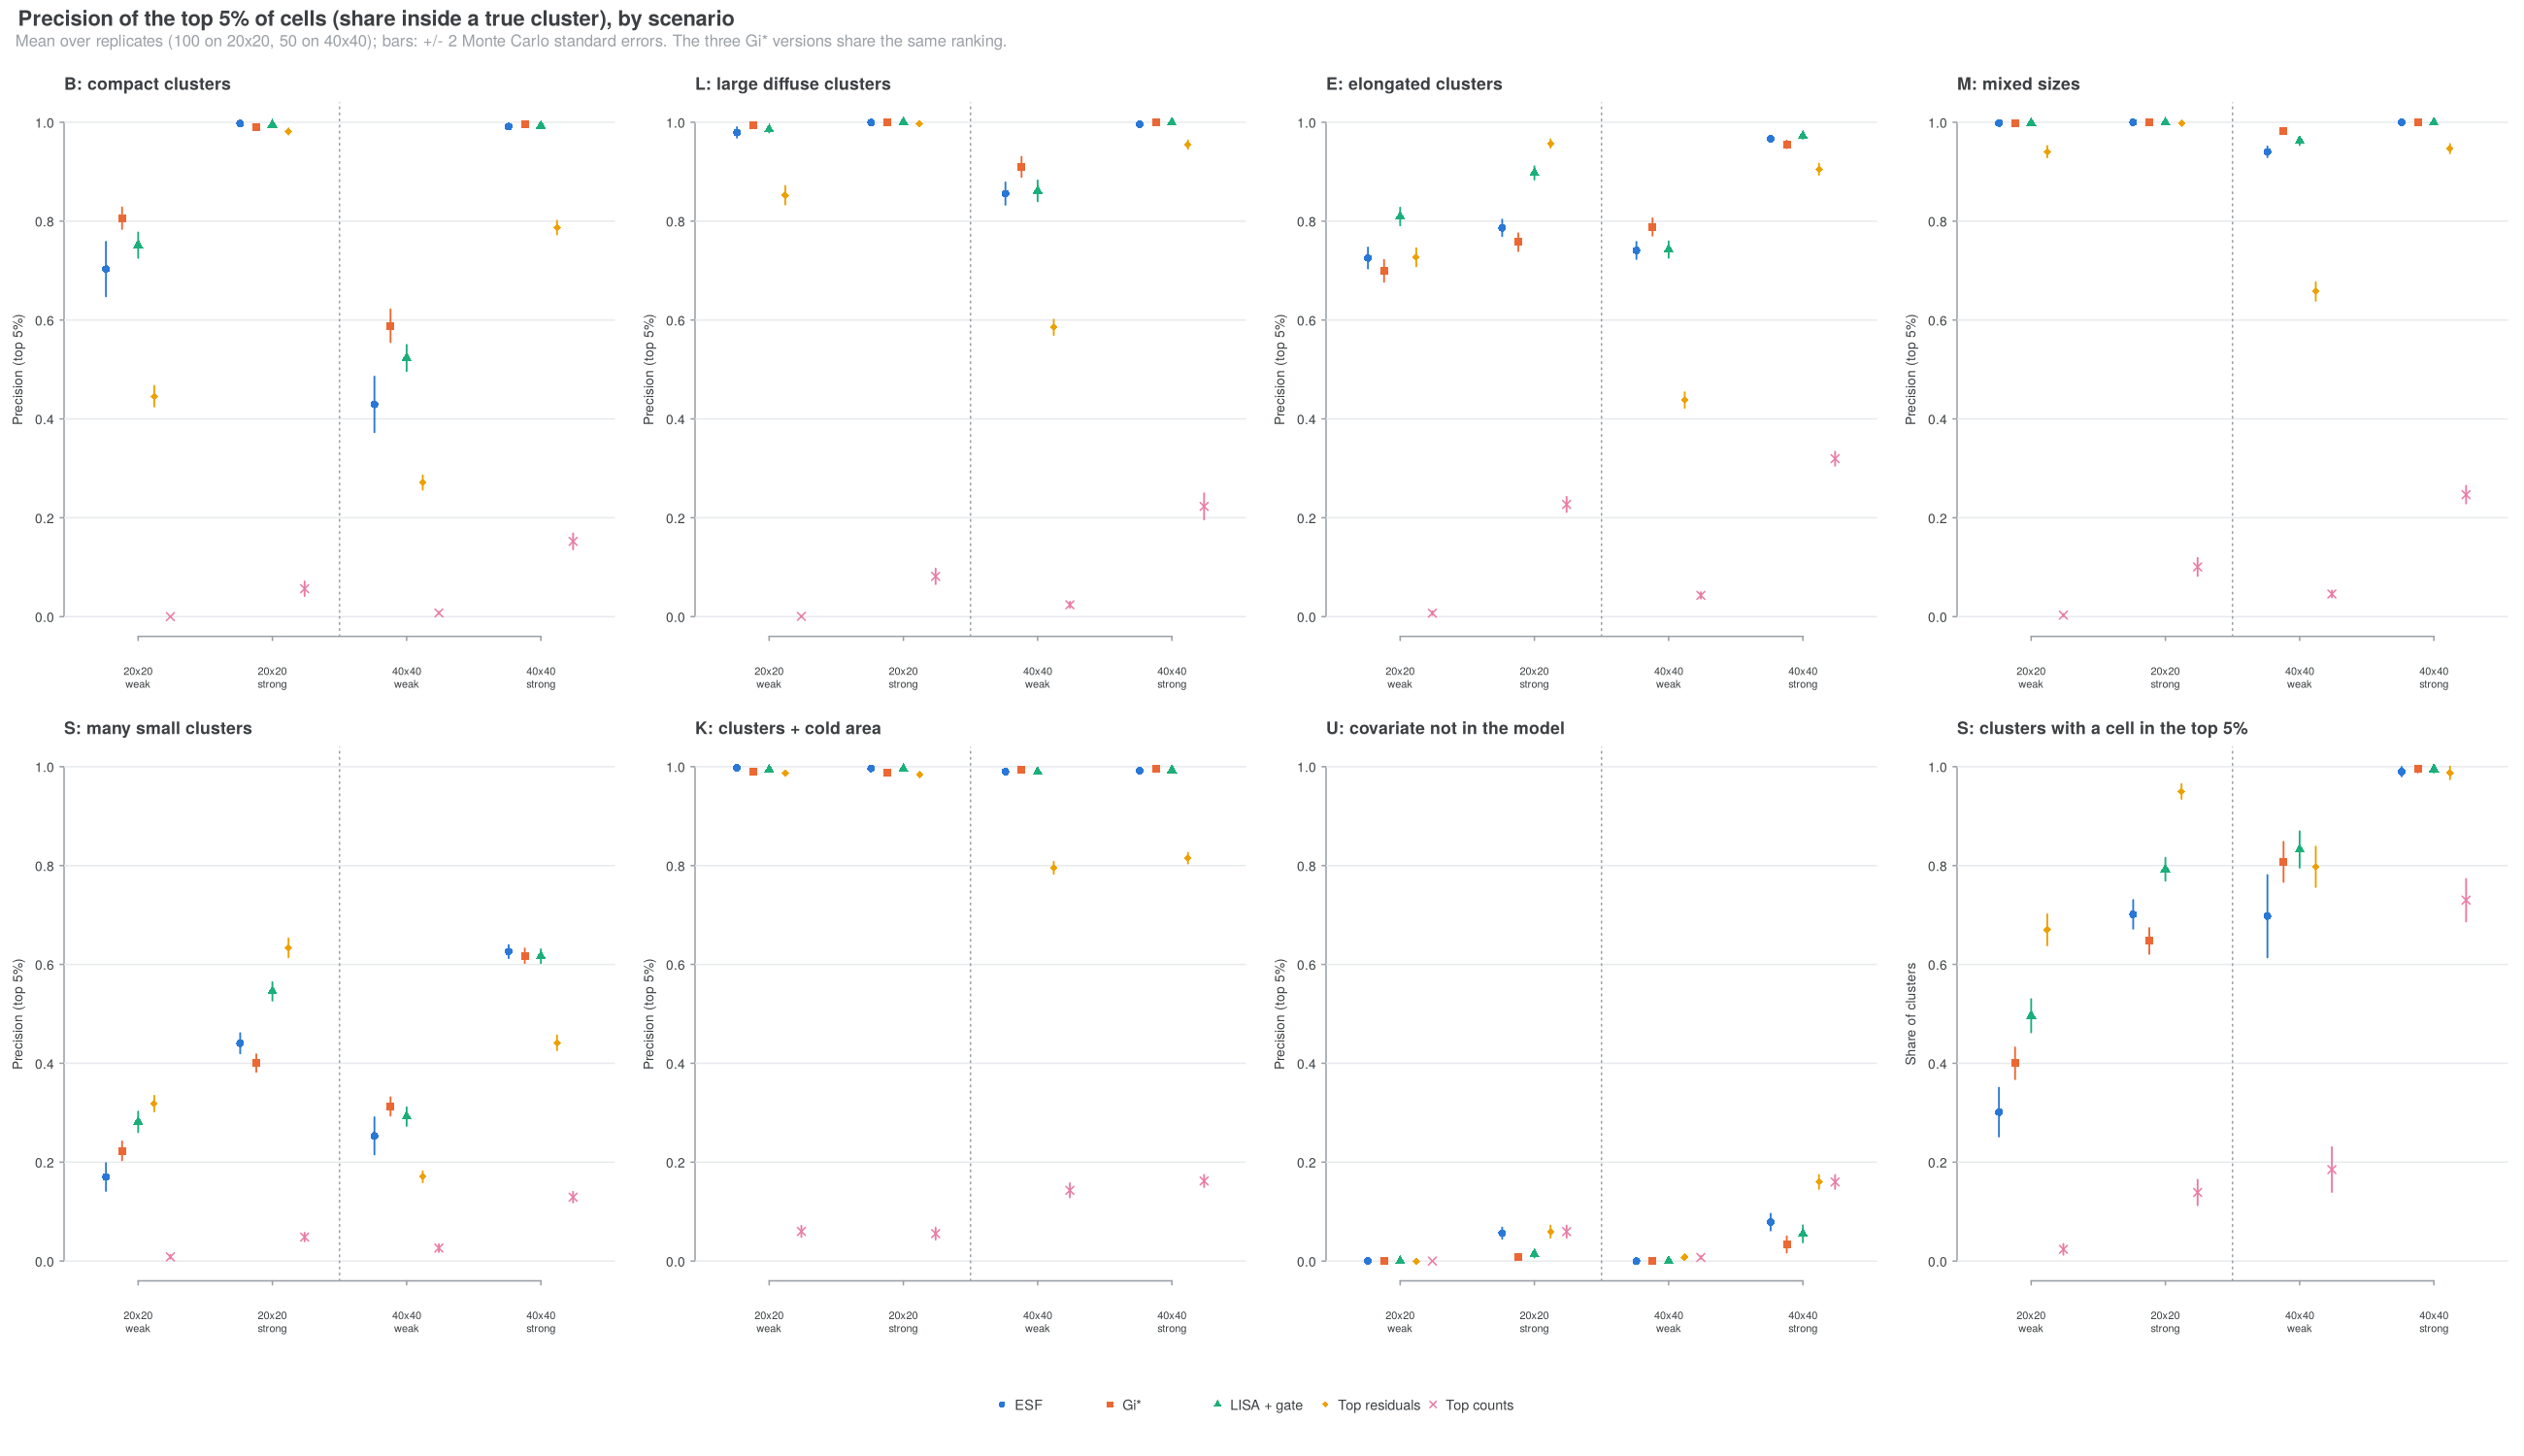
\includegraphics[width=\textwidth]{fig15_full_ranking.png}
\caption{Precision of the top 5\% of cells by scenario, grid and cluster strength; bars show $\pm2$ Monte Carlo standard errors. The last panel shows, for scenario S, the share of clusters with at least one cell in the top 5\%.}\label{fig:sim-ranking}
\end{figure}


%\paragraph{Labels.} 
Table~\ref{tab:sim-labels} and Figure~\ref{fig:sim-labels} summarise the hot and cold labels. With strong compact clusters, 78\% of the ESF hot cells belong to a cluster, against 67\% for $G_i^*$; with weak clusters the methods are within a few points of each other, and $G_i^*$ finds slightly more cluster cells. $G_i^*$ with the false discovery rate correction has the most precise labels (0.88--1.00) but finds few cluster cells when clusters are weak (1--15\%).

\begin{table}[ht]
\centering
\caption{Hot and cold labels, mean over replicates. Scenario U: lower is better.}\label{tab:sim-labels}
\small
\resizebox{\textwidth}{!}{\begin{tabular}{llrrrrr}
\toprule
Measure & Setting & ESF & Gi$^*$ & Gi$^*$ + gate & Gi$^*$ + gate + FDR & LISA + gate \\
\midrule
Hot cells inside a cluster & B strong 20$\times$20 & 0.78 & 0.67 & 0.67 & 0.88 & 0.76 \\
 & B weak 20$\times$20 & 0.60 & 0.63 & 0.62 & 0.97 & 0.68 \\
 & M strong 40$\times$40 & 0.93 & 0.91 & 0.91 & 0.99 & 0.94 \\
 & S weak 40$\times$40 & 0.28 & 0.28 & 0.29 & 1.00 & 0.31 \\
\addlinespace
Cluster cells labelled hot & B strong 20$\times$20 & 0.95 & 0.98 & 0.98 & 0.88 & 0.96 \\
 & B weak 20$\times$20 & 0.54 & 0.63 & 0.58 & 0.15 & 0.46 \\
 & M strong 40$\times$40 & 0.87 & 0.92 & 0.92 & 0.79 & 0.84 \\
 & S weak 40$\times$40 & 0.35 & 0.44 & 0.35 & 0.01 & 0.28 \\
\addlinespace
\% of cells hot, no clusters & C 20$\times$20 & 1.4 & 5.6 & 1.2 & 0.0 & 0.8 \\
 & N 20$\times$20 & 0.2 & 4.0 & 0.2 & 0.0 & 0.1 \\
 & C 40$\times$40 & 2.0 & 5.3 & 1.9 & 0.0 & 1.3 \\
 & N 40$\times$40 & 1.0 & 4.6 & 0.8 & 0.0 & 0.5 \\
\addlinespace
Cold cells inside the cold area & K strong 20$\times$20 & 0.81 & 0.70 & 0.70 & 0.88 & 0.81 \\
 & K strong 40$\times$40 & 0.62 & 0.58 & 0.58 & 0.93 & 0.74 \\
\addlinespace
Cold-area cells labelled cold & K strong 20$\times$20 & 0.97 & 1.00 & 1.00 & 0.96 & 0.98 \\
 & K strong 40$\times$40 & 0.87 & 0.96 & 0.96 & 0.80 & 0.85 \\
\addlinespace
Hot cells in the covariate area & U strong 20$\times$20 & 0.56 & 0.48 & 0.48 & 0.63 & 0.53 \\
 & U strong 40$\times$40 & 0.56 & 0.51 & 0.51 & 0.64 & 0.55 \\
\bottomrule
\end{tabular}
}
\end{table}



\begin{figure}[ht]
\centering
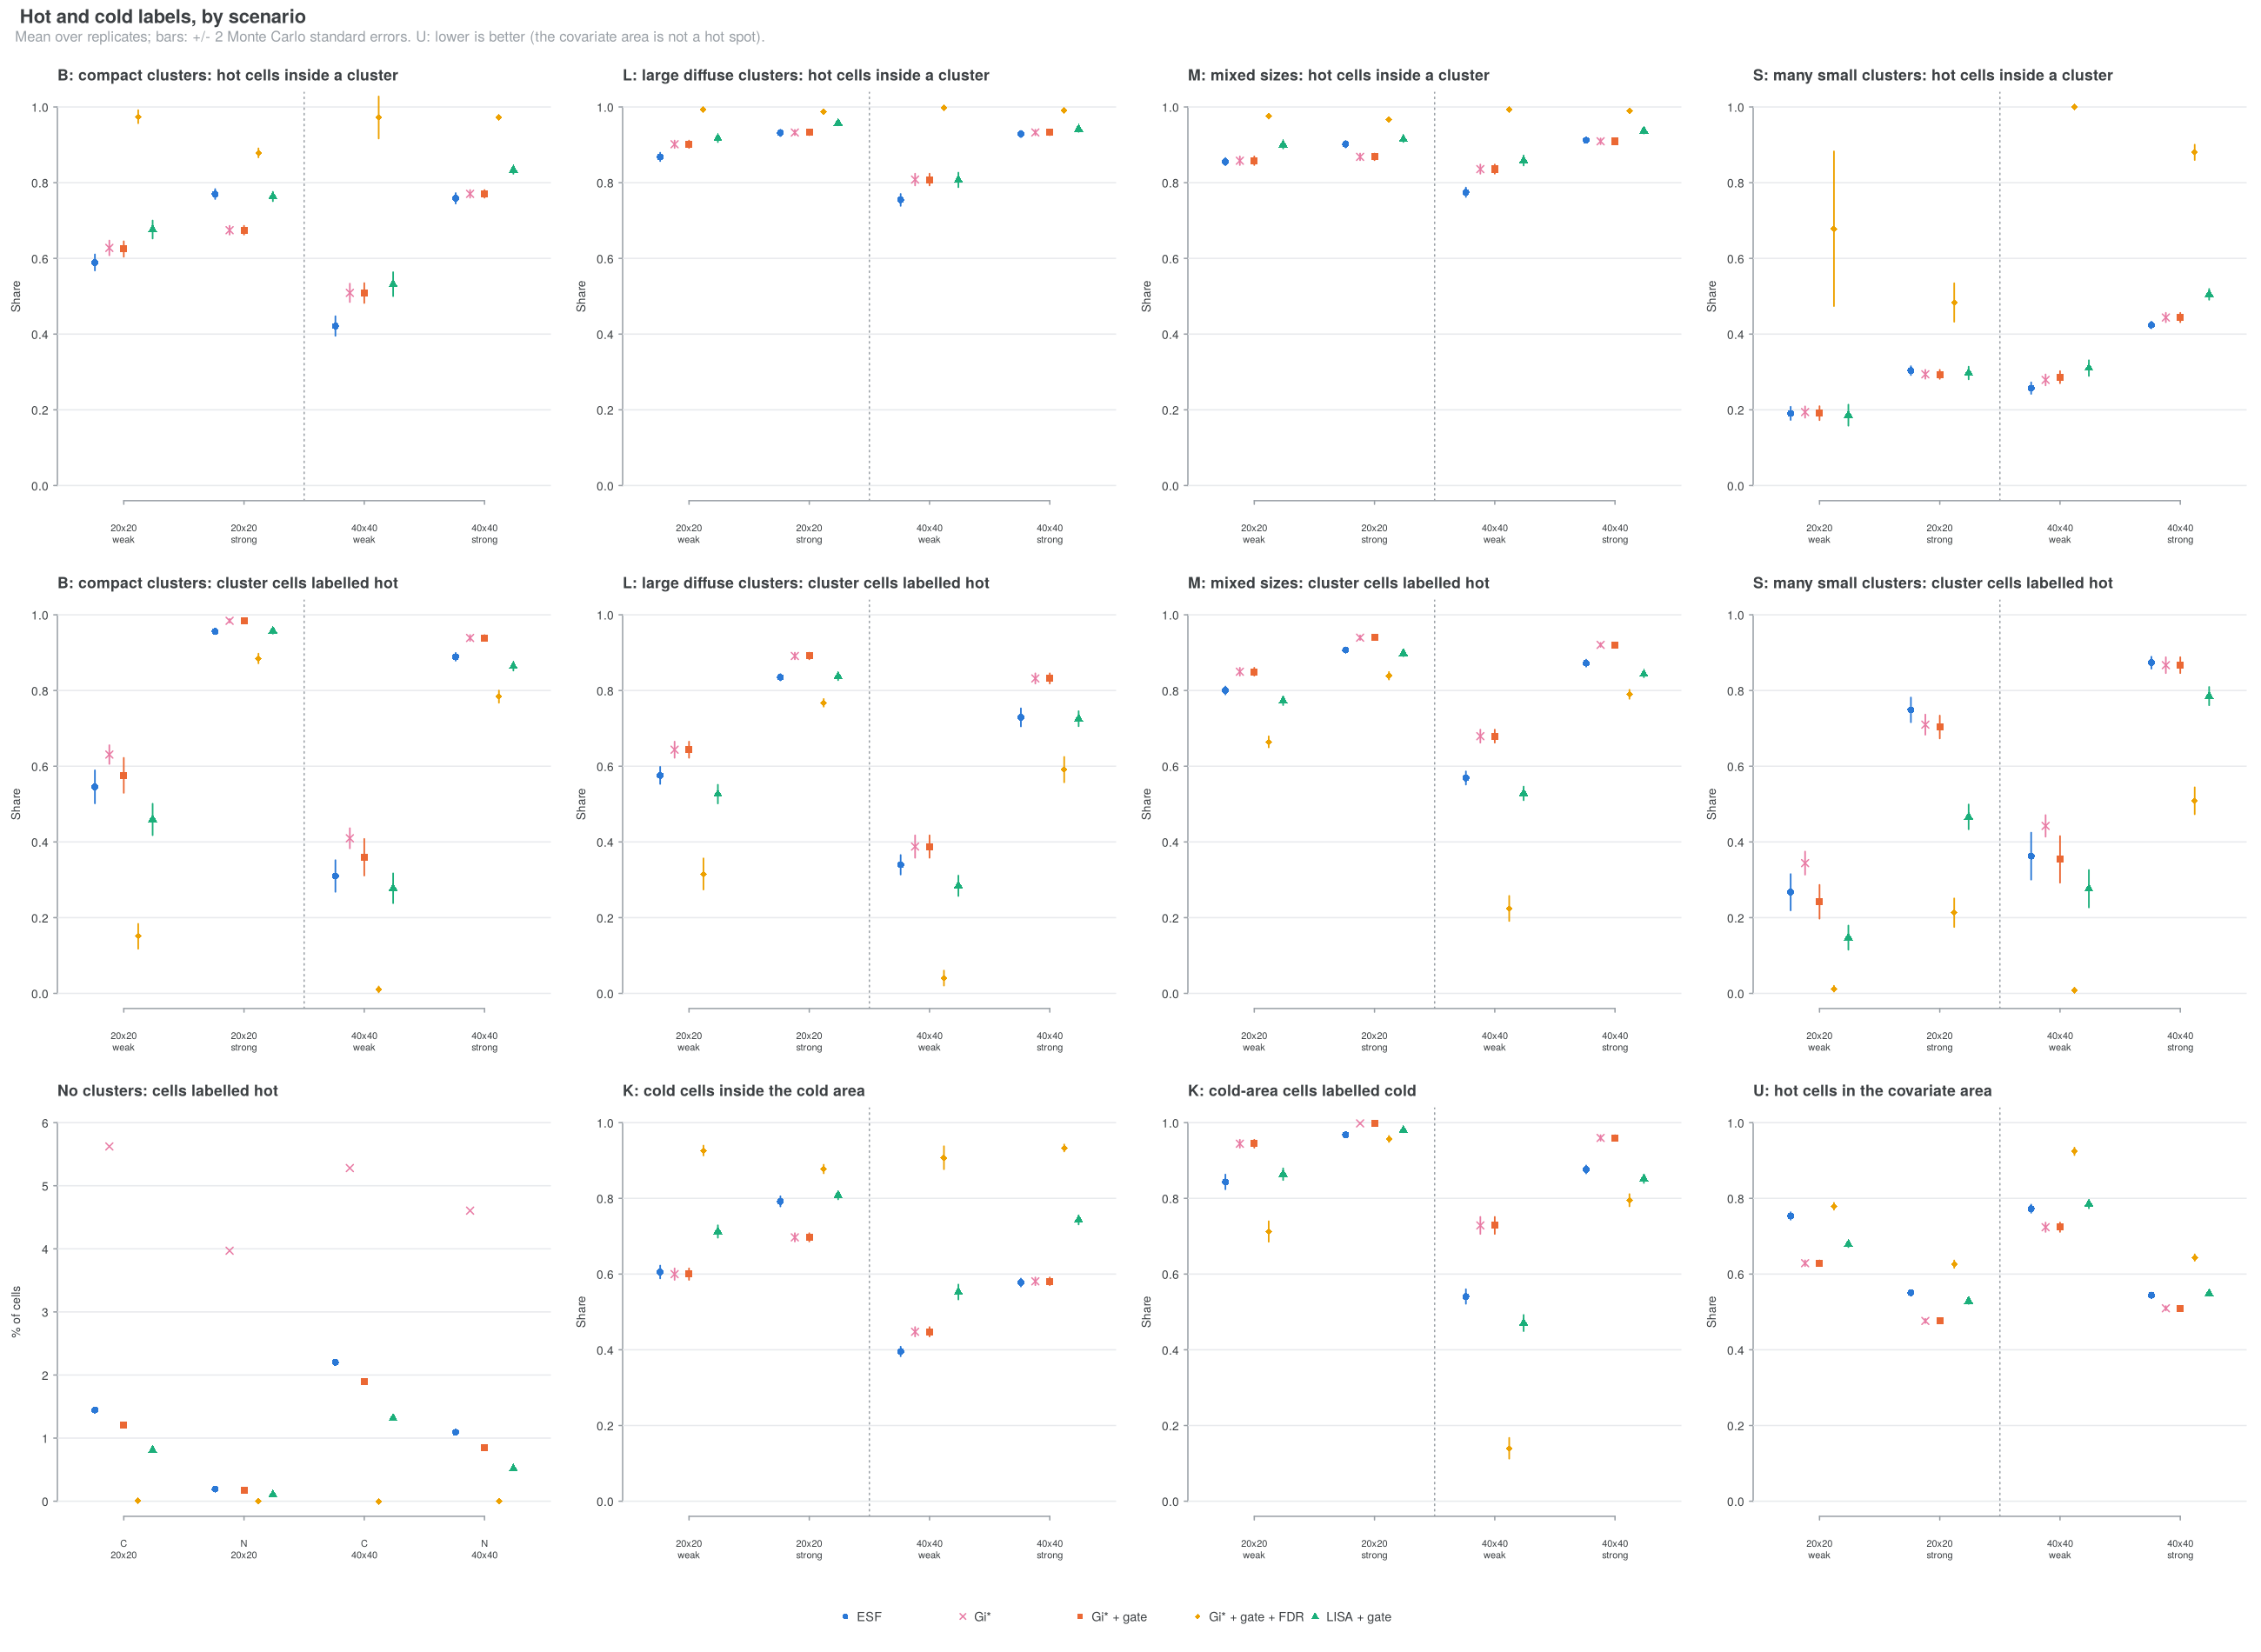
\includegraphics[width=\textwidth]{fig16_full_labels.png}
\caption{Hot and cold labels by scenario: share of hot cells inside a cluster, share of cluster cells labelled hot, percentage of the map labelled hot without clusters (C, N), cold labels in scenario K, and hot cells in the covariate area when the covariate is missing (U).}\label{fig:sim-labels}
\end{figure}


%\paragraph{No clusters.} 
Without the test of Step~1, $G_i^*$ labels 4.0--5.6\% of the map hot in scenarios C and N, as expected from its 5\% level. With the test, ESF labels 0.2--2.0\% hot, $G_i^*$ 0.2--1.9\% and LISA 0.1--1.3\%. The test therefore provides most of the protection against false hot spots, for all local methods. It rejects in 3\% of the datasets with random points on the $20\times20$ grid, and in 19\% (C, $20\times20$) and 32\% (C, $40\times40$) of the datasets that contain only the covariate area. The rejections in C occur because the covariate enters the model linearly while its effect on $\log(1+w)$ is not linear; a spline for each covariate reduced them to 4--6\%, at the cost of power with weak clusters (Section~\ref{sec:sim-choices}). On random points with the $40\times40$ grid the test rejected in 8 of 50 datasets; a check with 500 further datasets gave 5.0\% (95\% interval 3.3--7.3\%), so the test holds its level.

%\paragraph{Cold areas.} 
In scenario K with a strong cold area, ESF labels 97\% ($20\times20$) and 87\% ($40\times40$) of the cold-area cells cold, and 81\% and 62\% of its cold cells lie in the cold area. $G_i^*$ labels more of the cold area (100\% and 96\%), but a lower share of its cold cells lies inside it (70\% and 58\%); LISA has the most precise cold labels among the methods without the correction (81\% and 74\%). Outside the cold area, cold labels mark cells with few points by chance, which is more frequent on the finer grid.

%\paragraph{Missing covariate.}
 When the model does not receive the covariate (U), every method fails in the same way: about half of the hot cells (48--64\%) and most of the top 5\% (82--99\%) fall in the covariate area. A hot spot is only defined relative to the covariates that are in the model, which is why the choice of covariates in the application deserves care.



